

\begin{flushleft}
	Before starting with basic commands, let's first understand a few things.
	\paragraph{What is command prompt?}
	\begin{itemize}
		\item Command prompt is also known as shell prompt.
		\item Commands are entered in a terminal at the shell prompt. 
		\begin{figure}[h!]
			\centering
			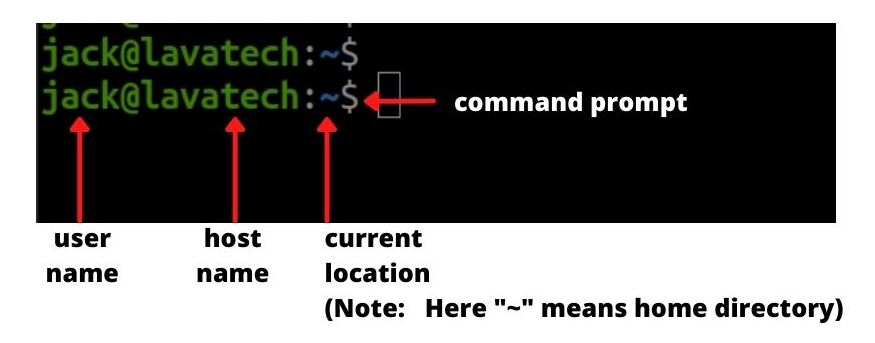
\includegraphics[scale=.5]{content/chapter2/images/command_prompt1.jpg}
			\caption{Command Prompt}
			\label{fig:command_prompt1}
		\end{figure}
		\begin{figure}[h!]
			\centering
			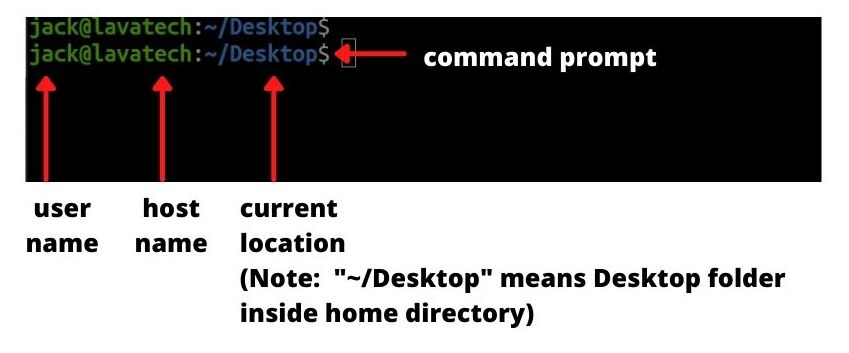
\includegraphics[scale=.5]{content/chapter2/images/command_prompt2.jpg}
			\caption{Command Prompt}
			\label{fig:command_prompt2}
		\end{figure}
		\item The shell prompt lists:
		\begin{itemize}
			\item Username who logged in
			\item Server hostname
			\item Current directory 
			\item \textbf{"\$"} prompt (if you are normal user) or \textbf{"\#"} prompt (if you are root user)
		\end{itemize}		
	

	\end{itemize}
		
	\newpage

	\paragraph{Command syntax}
	
	\begin{itemize}
		\item Commands entered at the shell prompt have three parts:
		\bigskip
			\begin{tcolorbox}[breakable,notitle,boxrule=-0pt,colback=pink,colframe=pink]
			\color{black}
			\fontdimen2\font=1em
			\bigskip
			Syntax:  command [options] [argument]
			\fontdimen2\font=4pt
			\bigskip
		\end{tcolorbox}
		Explaination:
		\begin{itemize}
			\item \textbf{command}: name of command
			\item \textbf{options}: start with one or two dashes (eg: -a or –all)
			\item \textbf{arguments}: a target that the command should operate on
			\item \textbf{"[]"} means optional.
		\end{itemize}

		\item
		Eg:
		\begin{figure}[h!]
			\centering
			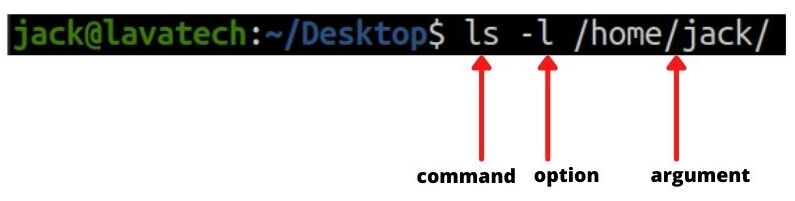
\includegraphics[scale=.65]{content/chapter2/images/command_prompt3.jpg}
			\caption{Command syntax}
			\label{fig:command_prompt3}
		\end{figure}
	\end{itemize}

	\newpage
	\paragraph{Now let's get started with some actual commands.}
	
	\begin{enumerate}
		\item \textbf{pwd}: Shows the user’s present working directory.
		\newline
		Eg:
		\begin{tcolorbox}[breakable,notitle,boxrule=-0pt,colback=black,colframe=black]
			\color{green}
			\fontdimen2\font=1em
			\# pwd
			\fontdimen2\font=4pt
		\end{tcolorbox}
		\bigskip
		\bigskip

		\item \textbf{clear}: Clears the contents of the screen.
		\newline	
		Eg:
		\begin{tcolorbox}[breakable,notitle,boxrule=-0pt,colback=black,colframe=black]
			\color{green}
			\fontdimen2\font=1em
			\# clear
			\fontdimen2\font=4pt
		\end{tcolorbox}
		\bigskip
		\begin{tcolorbox}[breakable,notitle,boxrule=-0pt,colback=orange,colframe=orange]
			\color{black}
			\textbf{Tip:} You can use the keyboard shortcut \textbf{CTRL+L} as well to clear the screen.
		\end{tcolorbox}
	
		\bigskip
		\bigskip
		
		\item \textbf{mkdir}: Create a directory.
		\bigskip
		\begin{tcolorbox}[breakable,notitle,boxrule=1pt,colback=pink,colframe=pink]
			\color{black}
			\fontdimen2\font=1em
			Syntax:  mkdir [options] foldername
			\fontdimen2\font=4pt
		\end{tcolorbox}
		Eg:
		\bigskip
		\begin{tcolorbox}[breakable,notitle,boxrule=-0pt,colback=black,colframe=black]
			\color{green}
			\fontdimen2\font=1em
			\# mkdir /home/jack/test
			\fontdimen2\font=4pt
		\end{tcolorbox}
		Option of \textbf{mkdir} command:
		\begin{itemize}
			\item -p: Creates a directory and all its parents too.
			\newline
			Eg:
			\begin{tcolorbox}[breakable,notitle,boxrule=-0pt,colback=black,colframe=black]
				\color{green}
				\fontdimen2\font=1em
				\# mkdir -p /home/jack/test/a/b/c
				\fontdimen2\font=4pt
			\end{tcolorbox}
		\end{itemize}
		\bigskip

		\item \textbf{ls}: Lists the content of a directory.
		\bigskip
		\begin{tcolorbox}[breakable,notitle,boxrule=1pt,colback=pink,colframe=pink]
			\color{black}
			\fontdimen2\font=1em
			Syntax:  ls [options] [foldername]
			\fontdimen2\font=4pt
		\end{tcolorbox}
	
		Eg:
		\bigskip
		\begin{tcolorbox}[breakable,notitle,boxrule=-0pt,colback=black,colframe=black]
			\fontdimen2\font=1em
			\color{yellow}
            \# List current directory content
            \newline
            \color{green}
			\# ls        
			\newline
			\newline
			\color{yellow}
			\# List content of /home directory
			\newline
			\color{green}
			\# ls /home                
			\fontdimen2\font=4pt
		\end{tcolorbox}
	
		Options with \textbf{ls} command-
		\begin{itemize}		
			\item \textbf{-l}: List more details of contents inside directory.
			\newline
			Eg:
			\begin{tcolorbox}[breakable,notitle,boxrule=-0pt,colback=black,colframe=black]
				\color{green}
				\$ ls -l /home
				\color{white}
				\small
				\fontdimen2\font=1em
				\newline
				total 24
				\newline
				drwxr-xr-x    3    jack   jack    4096 Feb2 17:02 jack
				\newline
				drwx------  2 root   root   16384 Dec8 14:39 lost+found
			\end{tcolorbox}
			Output explaination:
			\begin{itemize}
			\item Column 1 – Type \& permissions of file
				\item Column 2 - Number of links
				\item Column 3 - Owner of the file
				\item Column 4 - Group under which the file belongs
				\item Column 5 - Size of file
				\item Column 6 - Date of last update
				\item Column 7 – Last updated time of file
				\item Column 8 - Name of file/directory
			\end{itemize}
			\item \textbf{-d}: Shows information about directory rather than listing.
			\newline
			Eg:
			\begin{tcolorbox}[breakable,notitle,boxrule=-0pt,colback=black,colframe=black]
				\color{green}
				\# ls -ld 
				\color{white}
				%\small
				\fontdimen2\font=1em
				\newline
				drwxr-xr-x 3 jack jack 4096 Feb  2 17:02 .
				\fontdimen2\font=4pt
			\end{tcolorbox}
		
			\item \textbf{-a}: Shows all files, including hidden files. 
			\bigskip
			\begin{tcolorbox}[breakable,notitle,boxrule=-0pt,colback=yellow,colframe=yellow]
				\color{black}
				Note: Names of hidden files/folders begin with a dot.
			\end{tcolorbox}
			
			Eg:
			\begin{tcolorbox}[breakable,notitle,boxrule=-0pt,colback=black,colframe=black]
				\color{green}
				\fontdimen2\font=1em
				\# ls -a
				\color{white}
				\newline
				.  ..  .bash\_logout  .bashrc  Desktop  .profile
				\fontdimen2\font=4pt
			\end{tcolorbox}
		\end{itemize}
		\bigskip
		\bigskip

		\newpage
		\item \textbf{cd}: Used to switch between directories.
		\bigskip
		\begin{tcolorbox}[breakable,notitle,boxrule=1pt,colback=pink,colframe=pink]
			\color{black}
			\fontdimen2\font=1em
			Syntax:  cd [foldername]
			\fontdimen2\font=4pt
		\end{tcolorbox}
		Eg:
		\begin{tcolorbox}[breakable,notitle,boxrule=-0pt,colback=black,colframe=black]
			\fontdimen2\font=1em
			\color{yellow}
			\# \textbf{cd} without any argument \textbf{switch to user's home directory}.
			\newline
			\color{green}
			\# cd
			\fontdimen2\font=4pt
		\end{tcolorbox}
		Special characters that can be used with "cd" command:
		\begin{itemize}
			\item "." means current directory
			\item ".." means parent directory
			\item "–" would take you to previous working directory
			\item {"$\sim$"} would take you to home directory of the user
		\end{itemize}
		Eg:
		\begin{tcolorbox}[breakable,notitle,boxrule=-0pt,colback=black,colframe=black]
			\color{green}
			\fontdimen2\font=1em
			\# cd /home/
			\newline
			\# cd ..
			\newline
			\# cd -
			\newline
			\# cd {$\sim$}
			\fontdimen2\font=4pt
		\end{tcolorbox}

		\bigskip
		\bigskip
		\textbf{Absolute Path \& Relative Path}: 
		\begin{itemize}
			\item \textbf{Absolute path}: Starts with root directory (i.e "/") \& is complete path. 
			\item \textbf{Relative path}: It is relative to current location \& does not start with root directory (i.e "/").
			\begin{figure}[h!]
				\centering
				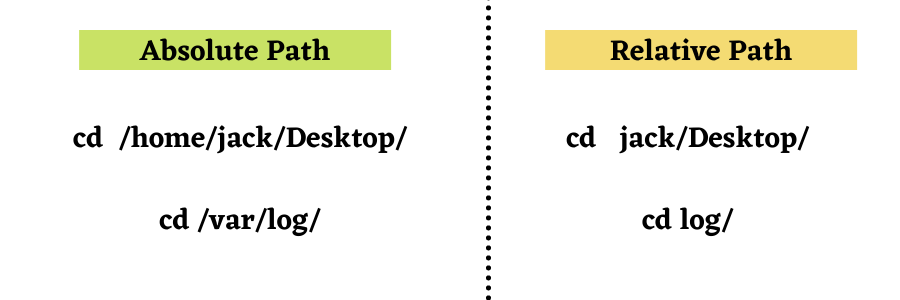
\includegraphics[scale=.45]{content/chapter2/images/path2.png}
				\caption{Absolute \& relative path}
				\label{fig:path2}
			\end{figure}	
		\end{itemize}
	
		\newpage		
		\item \textbf{cat}: Used to display contents of a file and also to create one.
		\begin{enumerate}[label=(\alph*)]
			\item Creating a file:
			\newline
			Eg:
			\begin{tcolorbox}[breakable,notitle,boxrule=-0pt,colback=black,colframe=black]
				\color{green}
				\fontdimen2\font=1em
				\# cat > hello.txt
				\newline
				hi
				\newline
				welcome to unix 
				\newline
				\color{yellow}
				\# End by pressing Ctrl + d
			\fontdimen2\font=4pt
			\end{tcolorbox}
			\item Displaying a file:
			\newline
			Eg:
			\begin{tcolorbox}[breakable,notitle,boxrule=-0pt,colback=black,colframe=black]
				\color{green}
				\fontdimen2\font=1em
				\# cat hello.txt
				\fontdimen2\font=4pt
			\end{tcolorbox}
		\end{enumerate}


		\bigskip
		\bigskip
		\item \textbf{touch}: Performs 2 functions:
		\begin{enumerate}[label=(\alph*)]
		\item Update timestamp of file, if it exists.
		\item Creates a new file, if it does not exists.
		\newline
		Eg:
		\begin{tcolorbox}[breakable,notitle,boxrule=-0pt,colback=black,colframe=black]
			\color{green}
			\fontdimen2\font=1em
			\# touch abc.txt
			\fontdimen2\font=4pt
		\end{tcolorbox}
		\end{enumerate}
		
		You can create multiple files using brace expansion.
		\newline
		Eg:
		\begin{tcolorbox}[breakable,notitle,boxrule=-0pt,colback=black,colframe=black]
			\color{green}
			\fontdimen2\font=1em
			\# touch {Sunday,Monday,Tuesday,Wednesday}.txt
			\newline
			\# touch file{1..3}.txt
			\newline
			\# touch file{a..h}.txt
			\newline
			\# touch file{a,b}{1,2}.txt
			\fontdimen2\font=4pt
		\end{tcolorbox}
		
		\bigskip
		\bigskip
		\item \textbf{cp}: Copy file or directory.
		\bigskip
		\begin{tcolorbox}[breakable,notitle,boxrule=1pt,colback=pink,colframe=pink]
			\color{black}
			\fontdimen2\font=1em
			Syntax: cp source destination
			\fontdimen2\font=4pt
		\end{tcolorbox}
		To copy multiple files to a directory:
			\bigskip
			\begin{tcolorbox}[breakable,notitle,boxrule=-0pt,colback=black,colframe=black]
				\color{green}
				\fontdimen2\font=1em
				\# cp file1 file2 file3 backup
				\fontdimen2\font=4pt
			\end{tcolorbox}

		Options with \textbf{cp} command:
		\begin{enumerate}[label=(\alph*)]
				\item \textbf{-r}: Copy directories recursively including all its files and subdirectories.
				\newline
				Eg:
				\begin{tcolorbox}[breakable,notitle,boxrule=-0pt,colback=black,colframe=black]
					\color{green}
					\fontdimen2\font=1em
					\# cp -r folder1  newfolder
					\fontdimen2\font=4pt
			\end{tcolorbox}
			\item \textbf{Wildcard character "*"}: Copy all files starting with a specific name.
			\bigskip
			\begin{tcolorbox}[breakable,notitle,boxrule=-0pt,colback=black,colframe=black]
				\color{green}
				\fontdimen2\font=1em
				\# cp file* backup
				\fontdimen2\font=4pt
			\end{tcolorbox}
		\end{enumerate}
		\bigskip
		\bigskip		

		
		\item \textbf{mv}: Used to move or rename the file/folder.
		\bigskip
		\begin{tcolorbox}[breakable,notitle,boxrule=1pt,colback=pink,colframe=pink]
			\color{black}
			\fontdimen2\font=1em
			Syntax:  mv source destination
			\fontdimen2\font=4pt
		\end{tcolorbox}
		\begin{enumerate}[label=(\alph*)]
		\item Renames file(or directory) when the \textbf{location of source and destination is same.}
		\bigskip
		\begin{tcolorbox}[breakable,notitle,boxrule=1pt,colback=black,colframe=black]
			\color{green}
			\fontdimen2\font=1em
			\# mv old-file new-file
			\fontdimen2\font=4pt
		\end{tcolorbox}
		\item Moves a files/directory to different location if \textbf{source and destination is different.}
		\bigskip
		\begin{tcolorbox}[breakable,notitle,boxrule=-0pt,colback=black,colframe=black]
			\color{green}
			\fontdimen2\font=1em
			\# mv oldfile new-file-location
			\fontdimen2\font=4pt
		\end{tcolorbox}
		\end{enumerate}
		\bigskip
		\bigskip
	
		\item \textbf{rm}: Deletes one or more files/folders.
		\bigskip
		\begin{tcolorbox}[breakable,notitle,boxrule=1pt,colback=pink,colframe=pink]
			\color{black}
			\fontdimen2\font=1em
			Syntax:  rm filename
			\fontdimen2\font=4pt
		\end{tcolorbox}
		Eg:
		\begin{tcolorbox}[breakable,notitle,boxrule=-0pt,colback=black,colframe=black]
			\color{green}
			\fontdimen2\font=1em
			\# rm one.txt
			\fontdimen2\font=4pt
		\end{tcolorbox}
		Options with \textbf{rm} command:
		\begin{enumerate}[label=(\alph*)]
			\item \textbf{-r}: Remove directories and their contents recursively.
			\bigskip
			\begin{tcolorbox}[breakable,notitle,boxrule=-0pt,colback=black,colframe=black]
				\color{green}
				\fontdimen2\font=1em
				\# rm -r foldername
				\fontdimen2\font=4pt
			\end{tcolorbox}
		\end{enumerate}	
		\bigskip
		\bigskip
		\newpage
		\item \textbf{rmdir}: Deletes only empty directory.
		\bigskip
		\begin{tcolorbox}[breakable,notitle,boxrule=1pt,colback=pink,colframe=pink]
			\color{black}
			\fontdimen2\font=1em
			Syntax:  rmdir directory
			\fontdimen2\font=4pt
		\end{tcolorbox}
		Eg:
		\begin{tcolorbox}[breakable,notitle,boxrule=-0pt,colback=black,colframe=black]
			\color{green}
			\fontdimen2\font=1em
			\# rmdir /tmp/project/
			\fontdimen2\font=4pt
		\end{tcolorbox}
		\bigskip
		\bigskip
		\item \textbf{df}: df stands for \textbf{disk free}. Displays information about disk usage.
		\bigskip
		\begin{tcolorbox}[breakable,notitle,boxrule=1pt,colback=pink,colframe=pink]
			\color{black}
			\fontdimen2\font=1em
			Syntax:  df
			\fontdimen2\font=4pt
		\end{tcolorbox}
		Options with \textbf{df} command:
		\begin{enumerate}[label=(\alph*)]
			\item \textbf{-h}: Display disk-usage size in GBs, MBs etc.
			\newline
			Eg:
			\begin{tcolorbox}[breakable,notitle,boxrule=1pt,colback=black,colframe=black]
				\color{green}
				\fontdimen2\font=1em
				\# df -h
				\fontdimen2\font=4pt
			\end{tcolorbox}
			\item \textbf{-T}: Print filesystem of each partition.
			\newline
			Eg:
			\begin{tcolorbox}[breakable,notitle,boxrule=-0pt,colback=black,colframe=black]
				\color{green}
				\fontdimen2\font=1em
				\# df -T
				\fontdimen2\font=4pt
			\end{tcolorbox}
		\end{enumerate}	
		\bigskip
		\bigskip
		
		\end{enumerate}
\end{flushleft}

\newpage

